\documentclass{article}
\usepackage[utf8]{inputenc}
\usepackage{amsmath}
\usepackage{enumitem}
\usepackage{graphicx}


\title{IFT-209 Programmation Système — Devoir 1}
\author{Jihane Adjeb \\ Yanéric Roussy}
\date{7 Septembre 2025}

\begin{document}

\maketitle

\section*{Question 1}
Effectuez les conversions suivantes, où $X_B$ est un nombre en base $B$ et $N$ est un
nombre décimal:

\begin{enumerate}[label=\alph*), itemsep=2em]
    \item $6241,3557_{7} = N$
    
    \textbf{Solution:}
    \[
    \begin{aligned}
    N &= 6 \cdot 7^3 + 2 \cdot 7^2 + 4 \cdot 7^1 + 1 \cdot 7^0 + \left(3 \cdot 7^{-1} + 5 \cdot 7^{-2} + 5 \cdot 7^{-3} + 7 \cdot 7^{-4}\right) \\
    &= 2058 + 98 + 28 + 1 + 0.545 \\
    &= 2185.545
    \end{aligned}
    \]

    \item $9387,875 = X_{16}$
    
    \textbf{Solution:}
    Pour la partie entière $9387$:
    \[
    \begin{aligned}
    9387 \div 16 &= 586 \text{ reste } 11 \, (B) \\
    586 \div 16 &= 36 \text{ reste } 10 \, (A) \\
    36 \div 16 &= 2 \text{ reste } 4 \\
    2 \div 16 &= 0 \text{ reste } 2
    \end{aligned}
    \]

    Partie entière est $24AB_{16}$.

    Pour la partie fractionnaire $0,875$:
    \[
    0,875 \cdot 16 = 14 \quad (E)
    \]
    
    Réponse finale:
    \[
    9387,875_{10} = 24AB,E_{16}
    \]

    \newpage

    \item $A8,1_{11} = X_{5}$
    
    \textbf{Solution:}
    \[
    \begin{aligned}
    N &= 10 \cdot 11^1 + 8 \cdot 11^0 + 1 \cdot 11^-1 \\
    &= 110 + 8 + 0.9 \\
    &= 118.9
    \end{aligned}
    \]
    
    On transforme maintenant en base 5. \\
    Pour la partie entière $118$:
    \[
    \begin{aligned}
    118.9 \div 5 &= 23 \text{ reste } 3 \\
    23 \div 5 &= 4 \text{ reste } 3 \\
    4 \div 5 &= 0 \text{ reste } 4
    \end{aligned}
    \]

    Pour la partie fractionnaire $0,9$:
    \[
    \begin{aligned}
    0,875 \cdot 3 &= 2.7 \\
    0.7 \cdot 3 &= 2.1 \\
    0.1 \cdot 3 &= 0.3 \\
    0.3 \cdot 3 &= 0.9
    \end{aligned}
    \]

    Réponse finale:
    \[
    X_{5} = 433,\overline{2200}
    \]
    
    \item $31124,32_{5} = X_{25}$

    \textbf{Solution :}\\
    Puisque $25 = 5^2$, on regroupe les chiffres de la base 5 par paquets de 2 (à partir de la droite):
    \[
    31124,32_{5} = [03]\,[11]\,[24],[32]_{5}
    \]

    Calculons la valeur de chaque groupe (en base 10):

    \[
    \begin{aligned}
    [03]_5 &= 0\cdot5^1 + 3\cdot5^0 = 3\\
    [11]_5 &= 1\cdot5^1 + 1\cdot5^0 = 6\\
    [24]_5 &= 2\cdot5^1 + 4\cdot5^0 = 14 \, (E)\\
    [32]_5 &= 3\cdot5^1 + 2\cdot5^0 = 17 \, (H).
    \end{aligned}
    \]

    Ainsi, chaque groupe devient un seul chiffre en base 25 :
    \[
    31124,32_{5} = 3\;6\;14 .\,17_{25} = 36\mathrm{E},\mathrm{H}_{25}.
    \]

    Réponse finale :
    \[
    31124,32_{5} = 36\mathrm{E},\mathrm{H}_{25}
    \]


    \item $4C85B,1A_{12} = N_{10}$

    \textbf{Solution:}  
    Valeurs : $C = 12$, $B = 11$, $A = 10$.
    \[
    \begin{aligned}
    N &= 4 \cdot 12^4 + 12 \cdot 12^3 + 8 \cdot 12^2 + 5 \cdot 12^1 + 11 \cdot 12^0 \\
      &\quad + \left(1 \cdot 12^{-1} + 10 \cdot 12^{-2}\right) \\
    &= 82944 + 20736 + 1152 + 60 + 11 + 0.0833 + 0.0694 \\
    &= 104903.15
    \end{aligned}
    \]

    Réponse finale :
    \[
    4C85B,1A_{12} = 104903.15_{10}
    \]

    \item $LAME,DUDE_{27} = X_{9}$

    \textbf{Solution:} \\
    On remarque que la lettre $U$ correspond à la valeur $30$.  
    Or, en base $27$, les chiffres possibles vont de $0$ à $26$.  
    Donc la présence de $U$ rend ce nombre \textbf{invalide en base 27}.  

    \item $6254,7001_{8} = X_{16}$

    \textbf{Solution:}  
    Conversion en base 2 (chaque chiffre octal → 3 bits) :
    \[
    6254,7001_{8} = 110\;010\;101\;100.111\;000\;000\;001_{2}
    \]

    Regroupons en paquets de 4 bits pour base 16 :
    \[
    1100\;1010\;1100.1110\;0000\;0001_{2} = C\;A\;C.E0\;1_{16}
    \]

    Réponse finale :
    \[
    6254,7001_{8} = CAC.E01_{16}
    \]
\end{enumerate}

\newpage

\section*{Question 2}
Effectuer les opérations suivantes, où XB est un nombre en base B. Vous devez faire
les opérations dans la base B:

\begin{enumerate}[label=\alph*), itemsep=2em]

  \item  $101110111,10011010_{2} + 10011,00011_{2} = X_{2}$
  
  \textbf{Solution:}
  \begin{figure}[h!]
    \centering
    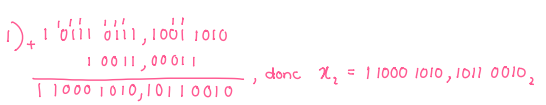
\includegraphics[width=1\textwidth]{images/binary_addition_q3_1.png}
  \end{figure}
  \\

  \item $714,2_{8} - 523,7_{8} = X_{8}$
 
  \textbf{Solution:}
  \begin{figure}[h!]
    \centering
    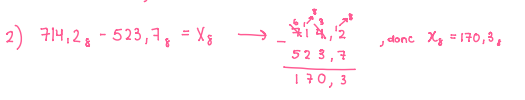
\includegraphics[width=1\textwidth]{images/octonary_substraction_q3_2.png}
  \end{figure}

  \item $714,2_{8} - 523,7_{8} = X_{8}$
 
  \textbf{Solution:}
  \begin{figure}[h!]
    \centering
    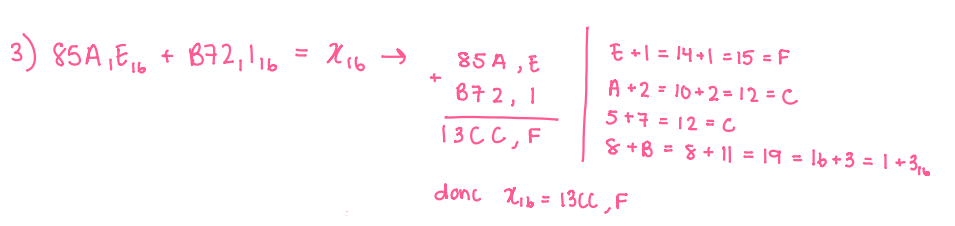
\includegraphics[width=1\textwidth]{images/hexadecimal_addition_q3_3.png}
  \end{figure}

  \newpage

  \item $4312_{5} - 1324_{5} = X_{5}$
 
  \textbf{Solution:}
  \begin{figure}[h!]
    \centering
    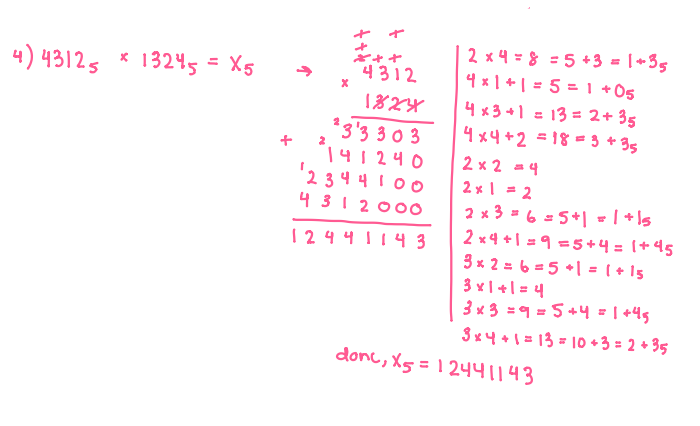
\includegraphics[width=1\textwidth]{images/quinary_multiplication_q3_4.png}
  \end{figure}

  \item $3683_{9} = X_{6}$
 
  \textbf{Solution:}
  \begin{figure}[h!]
    \centering
    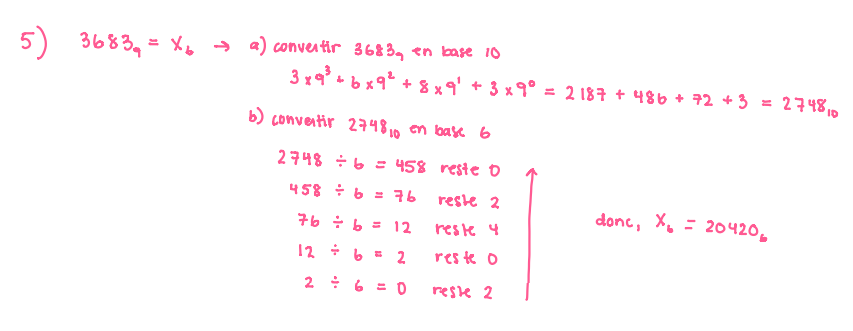
\includegraphics[width=1\textwidth]{images/senary_conversion_q3_5.png}
  \end{figure}

\end{enumerate}


\newpage

\section*{Question 3}
Quelle est la valeur maximale d'un nombre en base 15 exprimé grâce à 7 symboles?
Écrivez votre réponse en base 15 puis convertissez-la en base 10. \\[4pt]

\textbf{Solution:} \\[4pt]
On sait que la valeur maximale d'une base est (num. base) - 1. Donc dans notre cas:

\begin{flushleft}
\[
\begin{aligned}
&15 - 1 = 14 \rightarrow E \quad \text{plus qu'à écrire le nb. de symboles maximum:} \\
& EEEEEEE\text{,} \,\,\, \text{regardons le résultat en base 10 (N)}
\end{aligned}
\]
\end{flushleft}

\[
\begin{aligned}
N &= 14 \cdot 15^6 + 14 \cdot 15^5 + 14 \cdot 15^4 + 14 \cdot 15^3 + 14 \cdot 15^2 + 14 \cdot 15^1 + 14 \cdot 15^0 \\
&= 170\,859\,374
\end{aligned}
\]

\newpage

\section*{Question 4}
On définit une valeur entière positive $0 \leq n \leq 2^{32} - 1$
comme étant \emph{non discriminante} si, une fois décomposée en une suite d’octets, 
elle ne permet pas de distinguer entre le format \emph{big-endian} et le format \emph{little-endian}. 
Les valeurs non-discriminantes sont nécessairement des palindromes au niveau des octets.

\begin{enumerate}
    \item[a)] Si on exprime un mot de 32 bits de la façon suivante : ABCD
    où chaque lettre représente un octet, exprimez mathématiquement les conditions 
    qui vérifieront si ce mot est une valeur non-discriminante ou non.

    \textbf{Solution:}
    \begin{figure}[h!]
      \centering
      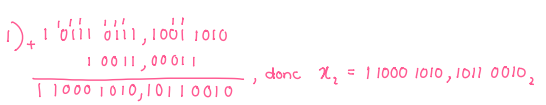
\includegraphics[width=1\textwidth]{images/binary_addition_q3_1.png}
    \end{figure}

    \item[b)] Quelle est, dans l’intervalle [25,\; 4\,278\,190\,123],
    la plus petite valeur non discriminante, ainsi que la plus grande valeur non discriminante ?

    \textbf{Raisonnement :}

Pour qu’une valeur de 32 bits soit \emph{non discriminante}, il faut qu’elle reste identique lorsqu’on inverse l’ordre des octets. 
Autrement dit, la suite d’octets doit former un palindrome. 
Si l’on note les octets $A$, $B$, $C$, $D$, alors la condition est
\[
ABCD = DCBA.
\]

Ainsi, pour un mot de 32 bits, il suffit que
\[
A = D \quad \text{et} \quad B = C.
\]
Autrement dit, la structure est de la forme
\[
ABBA.
\]

Chaque lettre ($A$, $B$) correspond à un octet, donc un entier compris entre $0$ et $255$ (représentation sur 8 bits).

\medskip

On cherche maintenant la plus petite et la plus grande valeur non discriminante dans l’intervalle
\[
[25,\; 4\,278\,190\,123].
\]

\medskip

\underline{Valeur minimale :}  
On ne peut pas prendre $A = B = 0$ (ce qui donnerait simplement $0$) car cela est inférieur à $25$.  
En augmentant légèrement les octets $B$ et $C$, on obtient la configuration :
\[
(A)\;0000\,0000 \quad (B)\;0000\,0001 \quad (B)\;0000\,0001 \quad (A)\;0000\,0000,
\]
c’est-à-dire
\[
0000\,0000\;0000\,0001\;0000\,0001\;0000\,0000.
\]

En décimal, cela donne
\[
65\,792.
\]

C’est donc la plus petite valeur non discriminante dans l’intervalle donné.

\medskip

\underline{Valeur maximale :}  
Pour maximiser la valeur, il faut prendre $A = 255$ et $B = 254$, ce qui donne
\[
(A)\;1111\,1111 \quad (B)\;1111\,1110 \quad (B)\;1111\,1110 \quad (A)\;1111\,1111,
\]
soit
\[
1111\,1111\;1111\,1110\;1111\,1110\;1111\,1111.
\]

En décimal, cela correspond à
\[
4\,278\,190\,078.
\]

\medskip

\textbf{Conclusion :}  
Dans l’intervalle considéré, la plus petite valeur non discriminante est
\[
65\,792,
\]
et la plus grande valeur non discriminante est
\[
4\,278\,190\,078.
\]

\end{enumerate}

\end{document}
